\documentclass[12pt,a4paper]{article}

% =========================================
% PAGE SETUP
% =========================================
\usepackage[
    a4paper,
    margin=25.4mm
]{geometry}


% =========================================
% BASIC PACKAGES
% =========================================
\usepackage{graphicx}       % Images
\usepackage{amsmath}        % Mathematics
\usepackage{amssymb}        % Mathematical symbols
\usepackage{booktabs}       % Professional tables
\usepackage{float}          % [H] figure/table positioning
\usepackage{caption}        % Caption customization
\usepackage{hyperref}       % Hyperlinks and references
\usepackage{ragged2e}       % Text alignment
\usepackage{setspace}       % Line spacing
\usepackage{hyperref}       % Clickable links and references
% =========================================
% APA REFERENCING
% =========================================

\usepackage[
    style=apa,
    backend=biber
]{biblatex}

\addbibresource{references.bib}


% =========================================
% HYPERLINK SETTINGS
% =========================================
\hypersetup{
    colorlinks=true,
    linkcolor=black,
    urlcolor=black,
    citecolor=black,
    pdftitle={Critical Research Review Article}
}

% Table and figure caption formatting
\DeclareCaptionFont{captionnine}{\fontsize{9pt}{11pt}\selectfont}

\captionsetup[table]{
    font=captionnine,
    justification=raggedright,
    singlelinecheck=false,
    labelsep=colon
}

\captionsetup[figure]{
    font=captionnine,
    justification=centering,
    singlelinecheck=false,
    labelsep=colon
}


% =========================================
% DOCUMENT
% =========================================
\begin{document}

\begin{center}

{\fontsize{18}{22}\selectfont\textbf{RESEARCH PROPOSAL}}

\vspace{0.5cm}

{\fontsize{18}{22}\selectfont\textbf{STANDARDISATION OF LEGAL REPORTING AND EMPIRICAL RELIABILITY METRICS FOR DIGITAL EVIDENCE}}

\vspace{1cm}

{\fontsize{12}{14}\selectfont\textbf{Group Members}}

\vspace{0.3cm}

{\fontsize{12}{14}\selectfont
1. Wan Wei Siang -- 251UC2508W\\
2. Elsa Zara Binti Fakhurrazi -- 251UC2502P\\
3. Terry Teoh Jay Poh -- 251UC2518F\\
4. Nur Afiqah Ramli -- 251UC2514E
}

\vspace{0.8cm}

{\fontsize{12}{14}\selectfont
\textbf{Programme:} [Programme Name]\\
\textbf{Course:} [Course Code and Course Name]\\
\textbf{Lecturer:} [Lecturer Name]\\
\textbf{Semester:} [Semester]\\
\textbf{Submission Date:} [Date]
}

\end{center}


% =========================================
% ABSTRACT
% =========================================

\vspace{0.5cm}

\noindent
\textbf{Abstract}

\vspace{0.2cm}

\begin{justify}

Write a concise summary of the entire review article. Write a concise summary of the entire review article. Write a concise summary of the entire review article. Write a concise summary of the entire review article.

Write a concise summary of the entire review article.Write a concise summary of the entire review article.Write a concise summary of the entire review article.






The abstract should include:

\begin{itemize}
    \item Background/context of the selected research topic
    \item Purpose of the review
    \item General approach used to select and analyse the research articles
    \item Major findings from the reviewed literature
    \item Key research gaps identified
    \item Overall conclusion
\end{itemize}

\textbf{Recommended length: 150--250 words.}

\vspace{0.3cm}

\textbf{Keywords:} Keyword 1; Keyword 2; Keyword 3; Keyword 4; Keyword 5

\end{justify}




% =========================================
% TABLE OF CONTENTS
% =========================================

\newpage

\tableofcontents

\newpage



% =========================================
% MAIN CONTENT
% =========================================

\begin{justify}

% =========================================
% 1. INTRODUCTION
% =========================================

\section{Introduction}

\subsection{Background}

Introduce the selected research topic and explain why it is important.

This is how you add inline references in the document given that all your references have been copied in the references.bib.
Recent studies have demonstrated the effectiveness of artificial
intelligence techniques \parencite{smith2024}.

Follow this example to include more than one references.Several studies have investigated these approaches
\parencite{smith2024,lee2023,ahmad2022}.

\vspace{0.5cm}
Discuss:

\begin{itemize}
    \item What is the research topic?
    \item What problem does it address?
    \item Why is the problem important?
    \item Where is the topic currently being applied?
    \item Why is there a need to study/review this topic?
\end{itemize}

Students should support important statements with appropriate research references.


\section{Literature Review (Recap)}

Clearly describe the problem or issue that motivates this literature review.

\vspace{0.5cm}
Explain:

\begin{itemize}
    \item What is currently known?
    \item What problems exist?
    \item What limitations exist in current approaches?
    \item Why is a review of existing research necessary?
\end{itemize}


\section{Problem Statement}

State the objectives of the review article.

\vspace{0.5cm}
For example:

\begin{enumerate}
    \item To review existing research related to [topic].
    \item To compare the approaches used by different researchers.
    \item To analyse the findings and limitations of existing studies.
    \item To identify research gaps and potential future research directions.
\end{enumerate}


\section{Research Questions}

Develop 2--4 research questions that guide the review.

\vspace{0.2cm}

For Example:


\textbf{RQ1:} What approaches have been used to address [research problem]?

\vspace{0.2cm}

\textbf{RQ2:} What are the major findings reported in existing studies?

\vspace{0.2cm}

\textbf{RQ3:} What are the limitations of the existing approaches?

\vspace{0.2cm}

\textbf{RQ4:} What research gaps and future opportunities can be identified?


% =========================================
% 2. REVIEW METHODOLOGY
% =========================================

\section{Review Methodology}

Explain how the group conducted the literature review.


\subsection{Literature Search Strategy}

Describe:

\begin{itemize}
    \item Databases/search engines used
    \item Search keywords
    \item Search strings
    \item Publication period
    \item Type of publications considered\newline
\end{itemize}


Example databases:

\begin{itemize}
    \item Scopus
    \item Web of Science
    \item IEEE Xplore
    \item ScienceDirect
    \item SpringerLink
    \item ACM Digital Library
    \item Google Scholar
\end{itemize}


\subsection{Inclusion and Exclusion Criteria}

Describe the criteria used to determine which research articles were included in or excluded from the review.

\textbf{Inclusion criteria may include:}

\begin{itemize}
    \item Articles directly related to the selected research topic
    \item Peer-reviewed research articles
    \item Articles published within the selected publication period
    \item Articles indexed in the selected academic databases
    \item Articles available in full text
\end{itemize}

\textbf{Exclusion criteria may include:}

\begin{itemize}
    \item Articles outside the scope of the research topic
    \item Duplicate publications
    \item Non-peer-reviewed publications
    \item Articles outside the selected publication period
    \item Articles without sufficient methodological or research information
\end{itemize}

\end{justify}

% =========================================
% SAMPLE TABLE
% =========================================

\begin{table}[H]
\caption{Inclusion and exclusion criteria used for the literature review}
\label{tab:inclusion-exclusion}

\fontsize{10pt}{12pt}\selectfont

\begin{tabular}{|p{4cm}|p{5cm}|p{5cm}|}
\hline
\centering\textbf{Criteria} &
\centering\textbf{Inclusion} &
\centering\textbf{Exclusion}
\tabularnewline
\hline

\centering Publication type &
\centering Peer-reviewed research articles &
\centering Non-peer-reviewed articles
\tabularnewline
\hline

\centering Publication period &
\centering [e.g., 2021--2026] &
\centering Articles outside selected period
\tabularnewline
\hline

\centering Language &
\centering English &
\centering Other languages
\tabularnewline
\hline

\centering Topic &
\centering Directly related to selected topic &
\centering Not directly related
\tabularnewline
\hline

\centering Full text &
\centering Full-text available &
\centering Full text unavailable
\tabularnewline
\hline

\end{tabular}

\end{table}

This is a sample table. Tables should be placed in the main text near to the first time they are cited, with the caption on top and left aligned. The font of the table caption is size 9 and the content in the table is size 10.



% =========================================
% SAMPLE FIGURE
% =========================================

\begin{figure}[H]
    \centering

    \fbox{%
        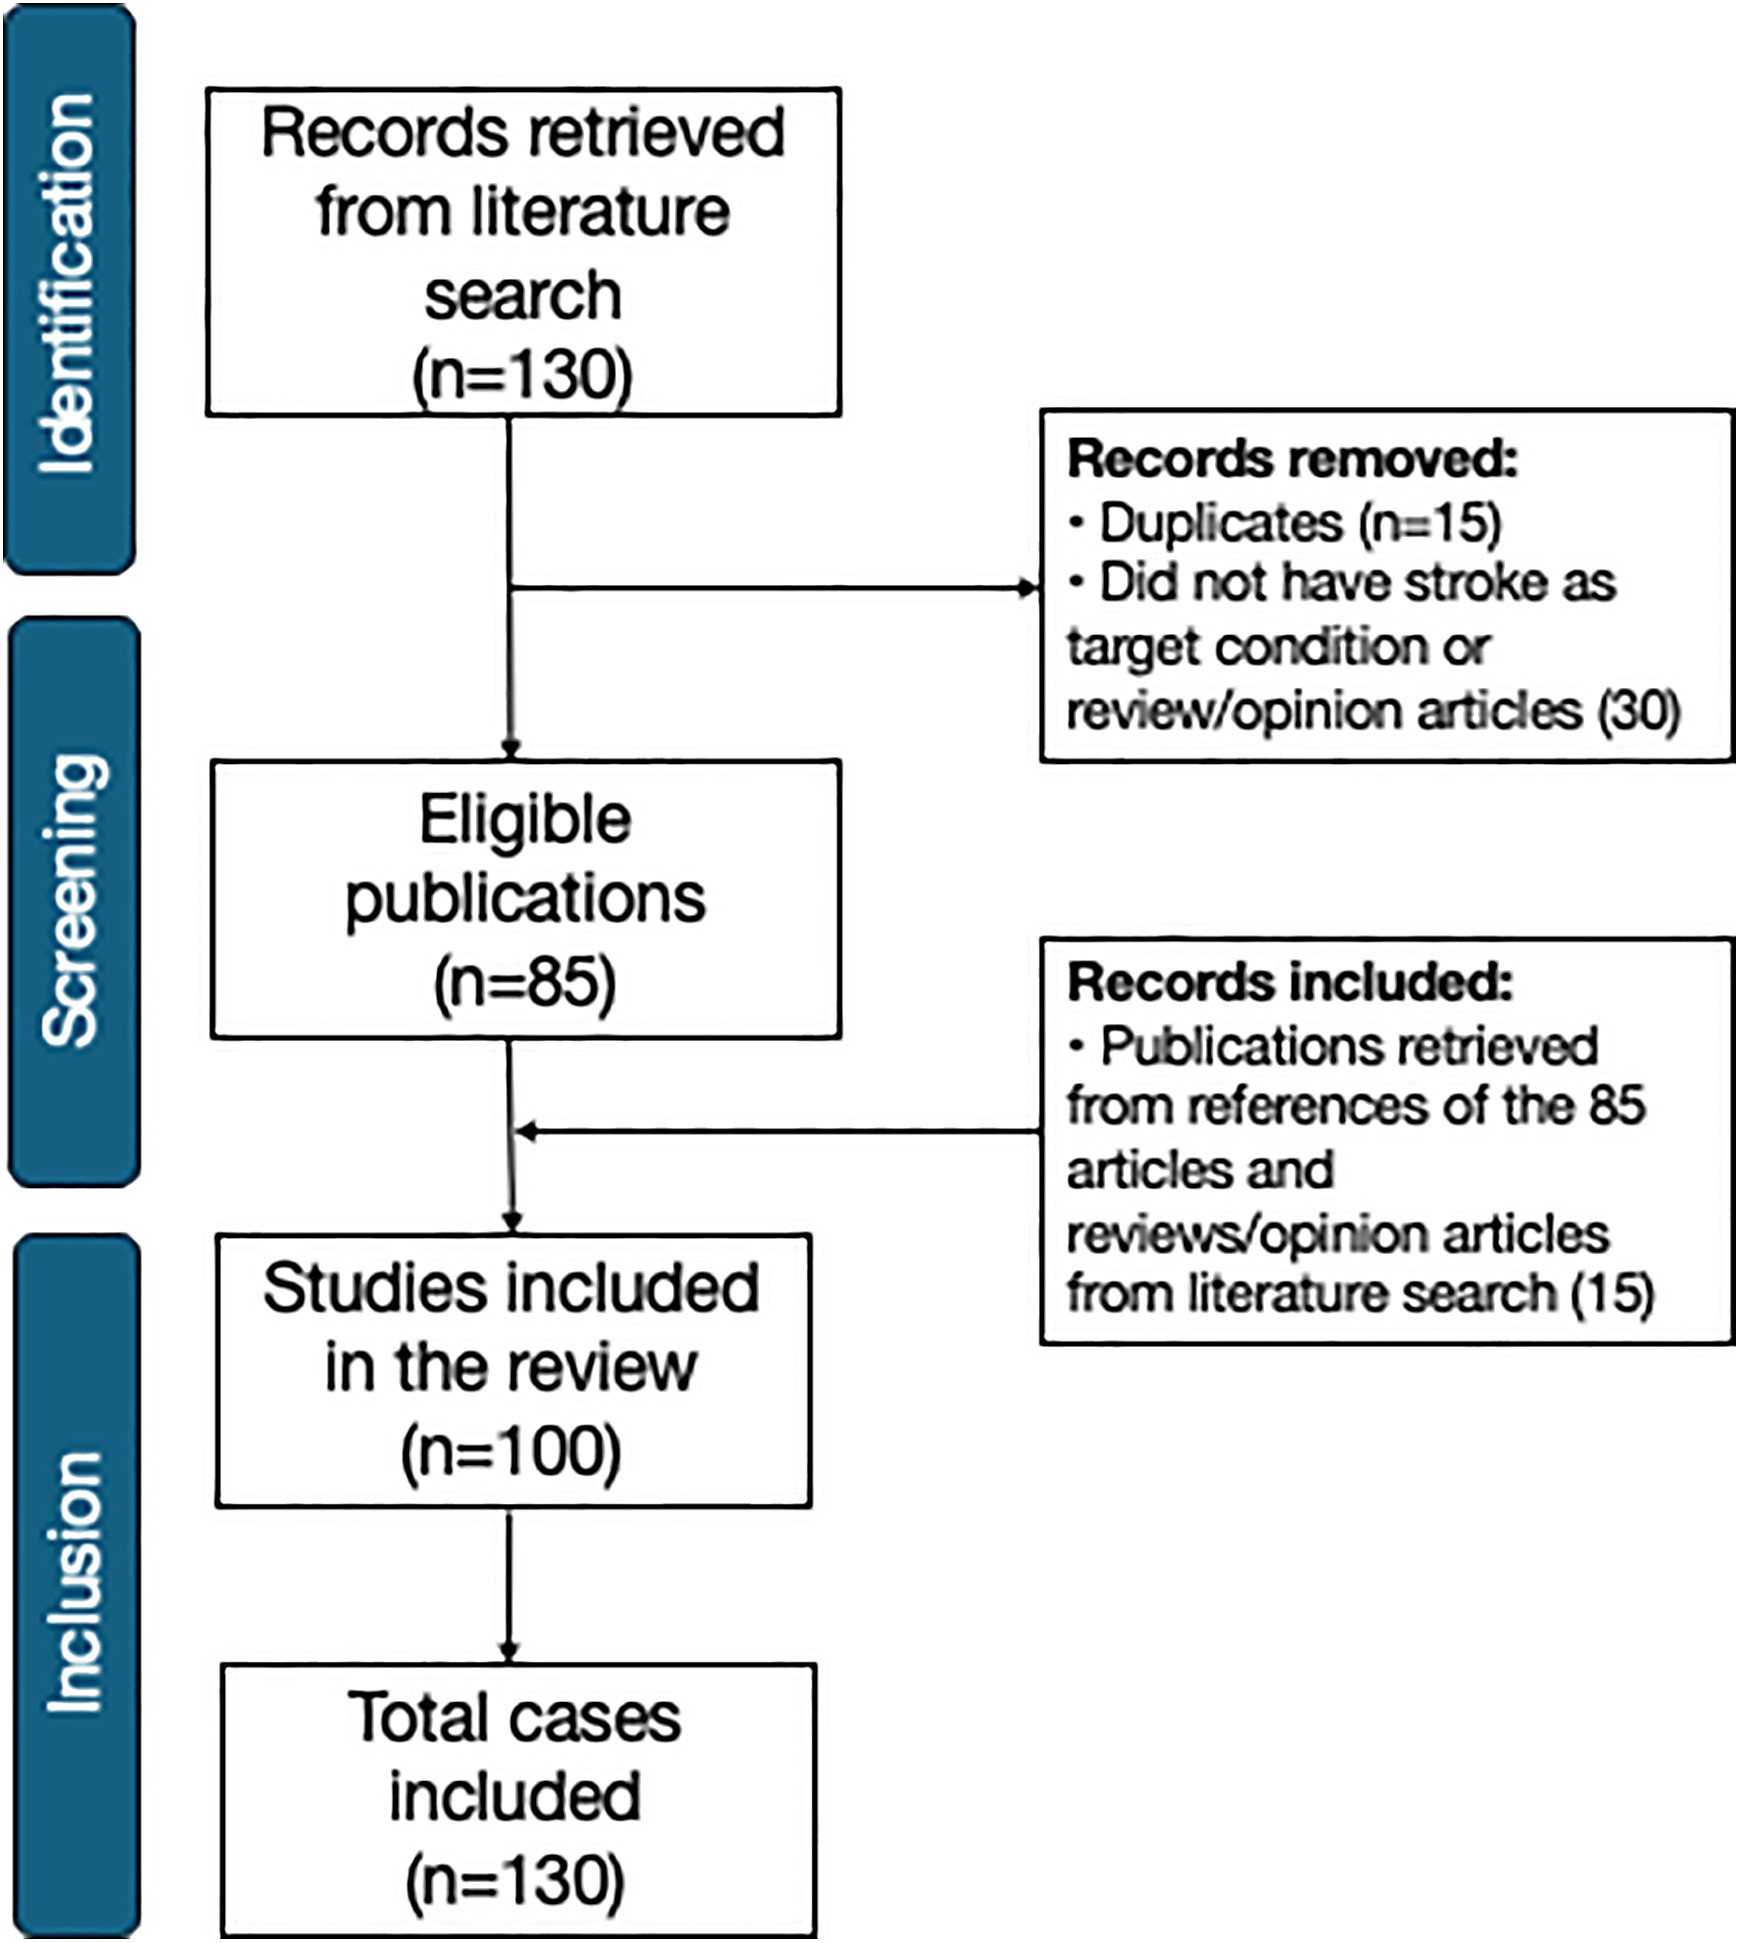
\includegraphics[width=0.80\textwidth]{figures/Prisma.jpg}%
    }

    \caption{PRISMA flow diagram of the study selection process.}
    \label{fig:prisma}
\end{figure}


This is a figure. All figures should be centred with figure caption following the sequence Figure 1, Figure 2, and so on. The caption should also be centred. The caption for figures should be size 9.



\subsection{Article Selection}

Each student must review \textbf{at least 3 research articles}.

Therefore:

\begin{itemize}
    \item \textbf{Minimum articles per student = 3}
    \item \textbf{Minimum articles per group = 12}
\end{itemize}

The group may use more than 12 articles if necessary.

Explain how the final articles were selected for the review.

% =========================================
% 8. DISCUSSION
% =========================================

\section{Expected Outcomes}

Provide an overall critical discussion of the literature.

The discussion should answer:

\begin{itemize}
    \item What has the research community achieved so far?
    \item Which approaches are most promising?
    \item What are the major challenges?
    \item Are the current approaches sufficient?
    \item What limitations remain?
    \item How has the research area evolved?
    \item What important issues remain unresolved?
\end{itemize}

This section should demonstrate \textbf{critical thinking}, not merely summarisation.

\section{Project Timeline}

Provide an overall critical discussion of the literature.

The discussion should answer:

\begin{itemize}
    \item What has the research community achieved so far?
    \item Which approaches are most promising?
    \item What are the major challenges?
    \item Are the current approaches sufficient?
    \item What limitations remain?
    \item How has the research area evolved?
    \item What important issues remain unresolved?
\end{itemize}

This section should demonstrate \textbf{critical thinking}, not merely summarisation.

% =========================================
% 9. CONCLUSION
% =========================================

\section{Conclusion}

Summarise the major findings of the review.

The conclusion should:

\begin{itemize}
    \item Restate the purpose of the review
    \item Summarise the major findings
    \item Highlight important research gaps
    \item State the overall conclusion
    \item Briefly indicate future research opportunities
\end{itemize}

Do not introduce completely new information or references in the conclusion.

% =========================================
% REFERENCES
% =========================================

\newpage

\phantomsection
\addcontentsline{toc}{section}{References}

\printbibliography[
    title={References}
]

\end{document}